\documentclass{article}
\usepackage[utf8]{inputenc}
\usepackage{graphicx}
\usepackage{parskip}
\usepackage{textcomp}
\usepackage{hyperref}
\hypersetup{
    colorlinks=true,
    linkcolor=blue,
    filecolor=magenta,      
    urlcolor=cyan,
}
\usepackage{listings}
\lstset{language=C,
                basicstyle=\ttfamily,
                keywordstyle=\color{blue}\ttfamily,
                stringstyle=\color{red}\ttfamily,
                commentstyle=\color{green}\ttfamily,
                morecomment=[l][\color{magenta}]{\#}
}

\title{GLCD Font and Graphic Creation - Tutorial}
\author{By \\ Umang Deshpande and Akshay Hegde}
\date{June 2017}

\begin{document}
\maketitle

\section{Software used}
\qquad \textit{Mikroelectronika GLCD Font Creator} is used for this purpose. GLCD Font Creator enables the creation of personalized fonts, symbols and icons for LCDs and GLCDs. Create fonts and symbols from scratch, or by importing existing fonts on your system. It lets you modify and adjust them for your needs, apply effects and finally export them as source code for use in mikroC, mikroBasic or mikroPascal compilers.

\subsection{Downloading and Installing Mikroelektronika GLCD Font Creator}
Download the Windows Installer from their \href{https://download.mikroe.com/setups/additional-software/glcd-font-creator/glcd-font-creator-v120.zip}{official website}. The Install Wizard is pretty straightforward. \\
For macOS, download the same .exe. Then use Wine to open it(Tutorials on installing and using Wine on macOS can be found \href{https://www.davidbaumgold.com/tutorials/wine-mac/}{here}). 

\section{Creating a font library}
\begin{enumerate}
    \item Upon double clicking on the .exe, the following window opens.
\begin{center}
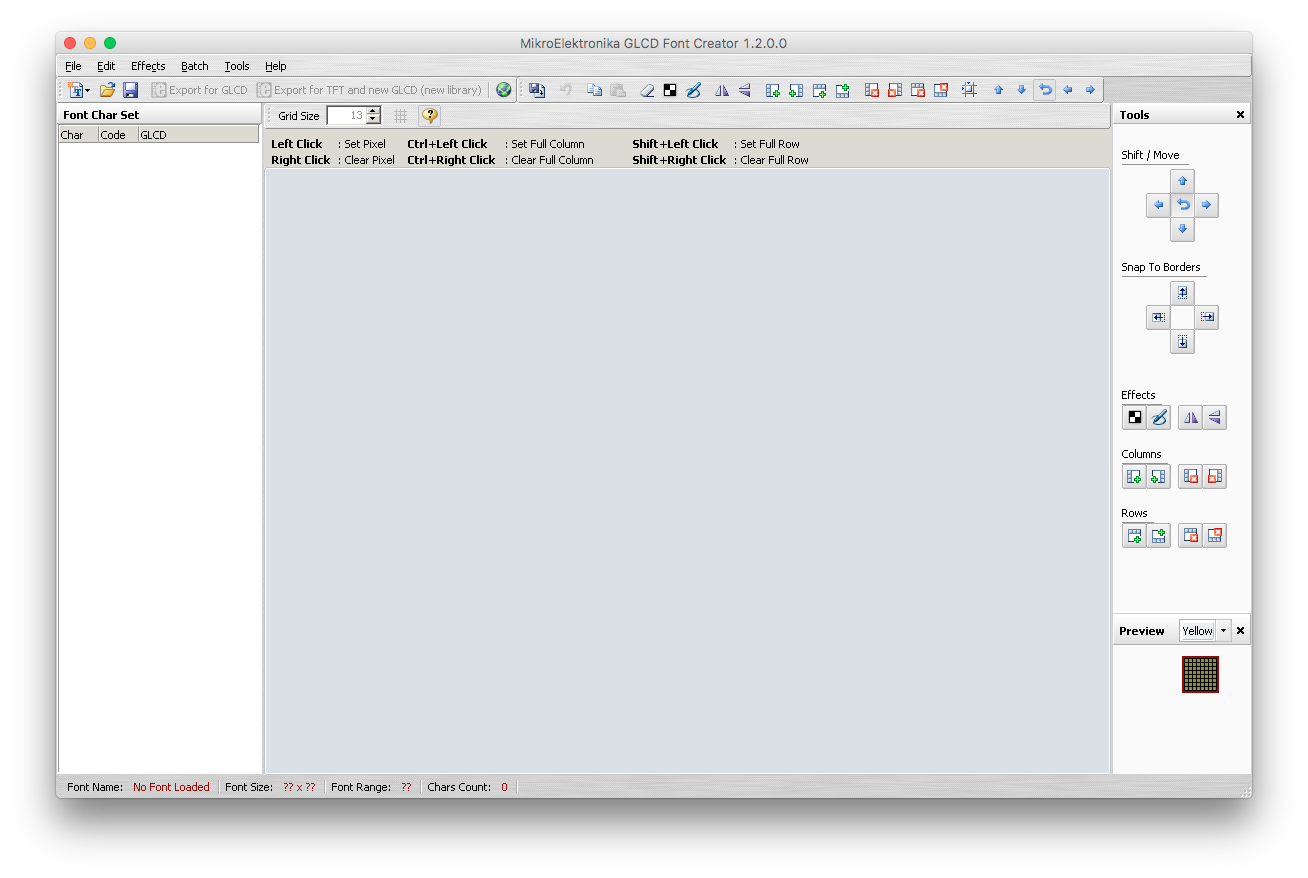
\includegraphics[width=12cm, height=7cm]{Screens/FontCreatorWindow} \\
\caption{Fig (a): Opening Window} \\
\end{center}
    \item Click on File-\>New Font-\>New Font From Scratch
    \item Set the parameters as shown:
\begin{center}
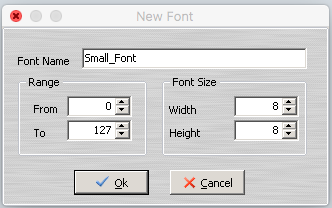
\includegraphics[width=5cm, height=3cm]{Screens/FontSetup} \\
\caption{Fig (b): Font parameters} \\
\end{center}
    \item Now, on the font char set plane, select each ASCII character and make the 8x8 pixel display for each in the workspace window. Example is as shown:\begin{center}
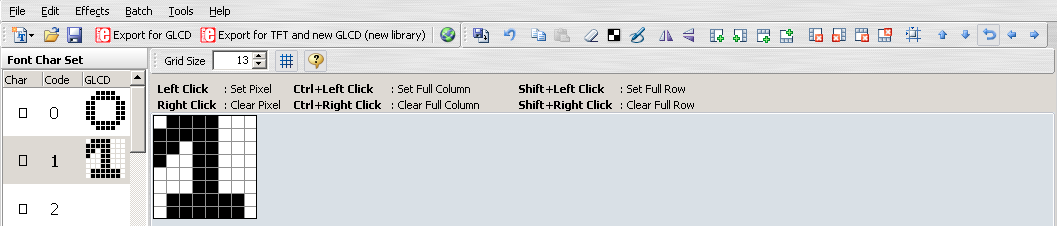
\includegraphics[width=12cm, height=3cm]{Screens/FontMaking} \\
\caption{Fig (c): Font Definition} \\
\end{center}
    \item Once, all the characters are done, click on export for GLCD button, then select mikroC compiler, and copy the code from the following window:
\begin{center}
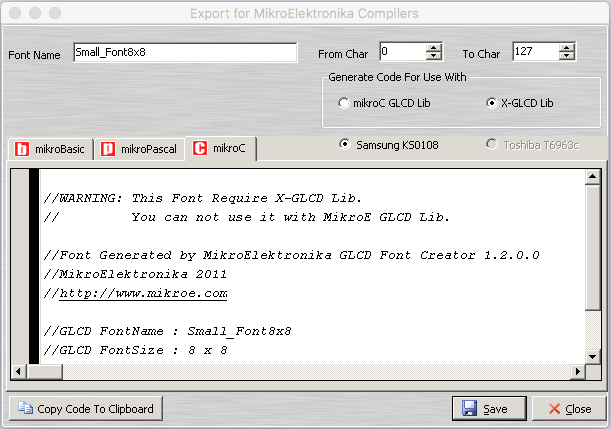
\includegraphics[width=8cm, height=8cm]{Screens/FontExporting} \\
\caption{Fig (d): Font export} \\
\end{center}
\qquad Thus, the font library has been created for use.
\end{enumerate}

\section{Creating a graphic}
\begin{enumerate}
    \item  For creating a graphic, in the window shown in Fig (b), the width is adjusted as required, and the height is kept identical(because the size of each page is 8 pixels in our GLCD). Now, across multiple characters the required graphic is created. For example, a larger D Font as follows:
\begin{center}
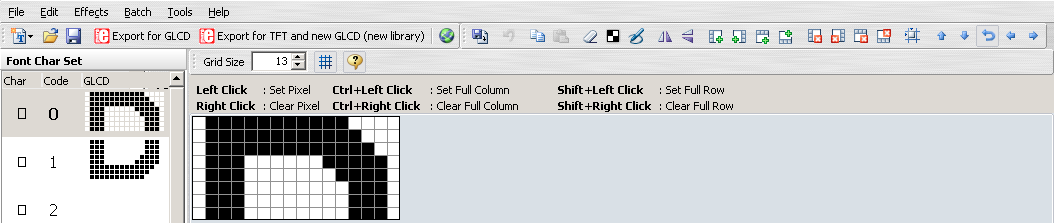
\includegraphics[width=12cm, height=3cm]{Screens/GraphicMaking} \\
\caption{Fig (d): Creating a larger GLCD graphic} \\
\end{center}
    \item The export process is identical to the font export, except that, only the characters across which the graphhic is created is exported.
\end{enumerate}
\end{document}
